\documentclass[tikz,border=0pt]{standalone}
\usepackage{amsmath, amssymb}
\usetikzlibrary{matrix, positioning, fit, backgrounds, calc}
\usepackage{helvet}
\usepackage{avant}
\renewcommand*\familydefault{\sfdefault}
\usepackage{textcomp}

\usepackage{fontspec}
\setmainfont{TeX Gyre Termes}
\setsansfont[
Path = fonts/,
UprightFont = *Medium.ttf,
BoldFont    = *Bold.ttf,
AutoFakeSlant = 0.2
]{GmarketSansTTF}
\begin{document}
	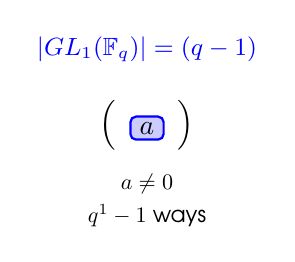
\begin{tikzpicture}[
		font=\sffamily,
		% Style for the matrices
		mtx/.style={
			matrix of math nodes,
			left delimiter=(, right delimiter=),
			nodes={minimum width=1.2em, inner sep=2pt, anchor=center},
			column sep=2pt, row sep=2pt,
			ampersand replacement=\&
		},
		% Highlighting styles for active columns
		hl-v1/.style={fill=blue!20, draw=blue, thick, rounded corners=2pt},
		hl-v2/.style={fill=orange!20, draw=orange, thick, rounded corners=2pt},
		hl-v3/.style={fill=green!20, draw=green!60!black, thick, rounded corners=2pt},
		hl-v4/.style={fill=purple!20, draw=purple, thick, rounded corners=2pt},
		% Style for the accumulating "Span Box"
		hl-span/.style={fill=gray!15, draw=gray, dashed, rounded corners=2pt},
		% Title & Text
		mainTitle/.style={font=\sffamily\bfseries\LARGE, color=darkgray, align=center},
		term label/.style={font=\bfseries\small, align=center}
		]
		
		% CASE m = 1
		\begin{scope}[shift={(-5, 4.5)}, scale=1]
			\node[term label, text=blue] at (0, 1) {$|GL_1(\mathbb F_q)| = \textcolor{blue}{(q-1)}$};
			\matrix[mtx] (M1) at (0, 0) {
				|[hl-v1]| a \\
			};
			\node[below=0.2cm of M1, align=center, scale=0.8] {
				$a\neq 0$ \\[1mm]
				\textbf{$q^1 - 1$} ways
			};
		\end{scope}
	\end{tikzpicture}
\end{document}